\documentclass[11pt,]{beamer}
\graphicspath{{img/}{./}}
\usepackage{booktabs} % \toprule, \midrule and \bottomrule
\usepackage{amsmath}
\usepackage{amssymb}
\usepackage{graphicx}
\usepackage{pdfpages}
\usepackage{xcolor}
\usepackage{hyperref}





%----------------------------------------------------------------------------------------
%	SELECT LAYOUT THEME
%----------------------------------------------------------------------------------------
%\usetheme{default}
%\usetheme{AnnArbor}
%\usetheme{Antibes}
%\usetheme{Bergen}
%\usetheme{Berkeley}
%\usetheme{Berlin}
%\usetheme{Boadilla}
%\usetheme{CambridgeUS}
%\usetheme{Copenhagen}
%\usetheme{Darmstadt}
%\usetheme{Dresden}
%\usetheme{Frankfurt}
%\usetheme{Goettingen}
%\usetheme{Hannover}
%\usetheme{Ilmenau}
%\usetheme{JuanLesPins}
%\usetheme{Luebeck}
\usetheme{Madrid}
%\usetheme{Malmoe}
%\usetheme{Marburg}
%\usetheme{Montpellier}
%\usetheme{PaloAlto}
%\usetheme{Pittsburgh}
%\usetheme{Rochester}
%\usetheme{Singapore}
%\usetheme{Szeged}
%\usetheme{Warsaw}

%----------------------------------------------------------------------------------------
%	SELECT COLOR THEME
%----------------------------------------------------------------------------------------

%\usecolortheme{albatross}
%\usecolortheme{beaver}
%\usecolortheme{beetle}
%\usecolortheme{crane}
%\usecolortheme{dolphin}
%\usecolortheme{dove}
%\usecolortheme{fly}
%\usecolortheme{lily}
%\usecolortheme{monarca}
%\usecolortheme{seagull}
%\usecolortheme{seahorse}
%\usecolortheme{spruce}
%\usecolortheme{whale}
%\usecolortheme{wolverine}

%----------------------------------------------------------------------------------------
%	SELECT FONT THEME & FONTS
%----------------------------------------------------------------------------------------

%\usefonttheme{default} % Typeset using the default sans serif font
\usefonttheme{serif} % Typeset using the default serif font (make sure a sans font isn't being set as the default font if you use this option!)
%\usefonttheme{structurebold} % Typeset important structure text (titles, headlines, footlines, sidebar, etc) in bold


%------------------------------------------------

\usepackage{lmodern}
%\usepackage{mathptmx} % Use the Times font for serif text
%\usepackage{palatino} % Use the Palatino font for serif text

%\usepackage{helvet} % Use the Helvetica font for sans serif text
%\usepackage[default]{opensans} % Use the Open Sans font for sans serif text
%\usepackage[default]{lato} % Use the Lato font for sans serif text

%----------------------------------------------------------------------------------------
%	SELECT INNER THEME
%----------------------------------------------------------------------------------------
%\useinnertheme{default}
\useinnertheme{circles}
%\useinnertheme{rectangles}
%\useinnertheme{rounded}
%\useinnertheme{inmargin}

%----------------------------------------------------------------------------------------
%	SELECT OUTER THEME
%----------------------------------------------------------------------------------------

%\useoutertheme{default}
%\useoutertheme{infolines}
%\useoutertheme{miniframes}
\useoutertheme{smoothbars}
%\useoutertheme{sidebar}
%\useoutertheme{split}
%\useoutertheme{shadow}
%\useoutertheme{tree}
%\useoutertheme{smoothtree}

%\setbeamertemplate{footline} % Uncomment this line to remove the footer line in all slides
%\setbeamertemplate{footline}[page number] % Uncomment this line to replace the footer line in all slides with a simple slide count

%\setbeamertemplate{navigation symbols}{} % Uncomment this line to remove the navigation symbols from the bottom of all slides

%----------------------------------------------------------------------------------------
%	PRESENTATION INFORMATION
%----------------------------------------------------------------------------------------

\title[Rotation of The Fluid Flow]{Rotation of The Fluid Flow}
\subtitle{A brief introduction of rotation of fluid}
\author[Chang-Mao Yang]{Chang-Mao Yang}

\institute[CCU]{\textit{Department of Physics, National Chung Cheng University}\\ \smallskip 409220055@alum.ccu.edu.tw}

\date[\today]{Final Project of \textit{Introduction to Fluid Mechanics} \\ \today}

%----------------------------------------------------------------------------------------

\begin{document}

%----------------------------------------------------------------------------------------
%	TITLE SLIDE
%----------------------------------------------------------------------------------------

\begin{frame}
	\titlepage
\end{frame}

%----------------------------------------------------------------------------------------
%	TABLE OF CONTENTS SLIDE
%----------------------------------------------------------------------------------------

\begin{frame}
	\frametitle{Presentation Overview}
	\tableofcontents
\end{frame}

%----------------------------------------------------------------------------------------
%	PRESENTATION BODY SLIDES
%----------------------------------------------------------------------------------------


%------------------------------------------------
\section{Curl and Rotation}
%------------------------------------------------
%----
\subsection{What is angular velocity?}
%----
\begin{frame}
\frametitle{What is the rotation of a particle?}
First we look at a moving particle in a space $\mathbb{R}^2$.
	\begin{figure}
    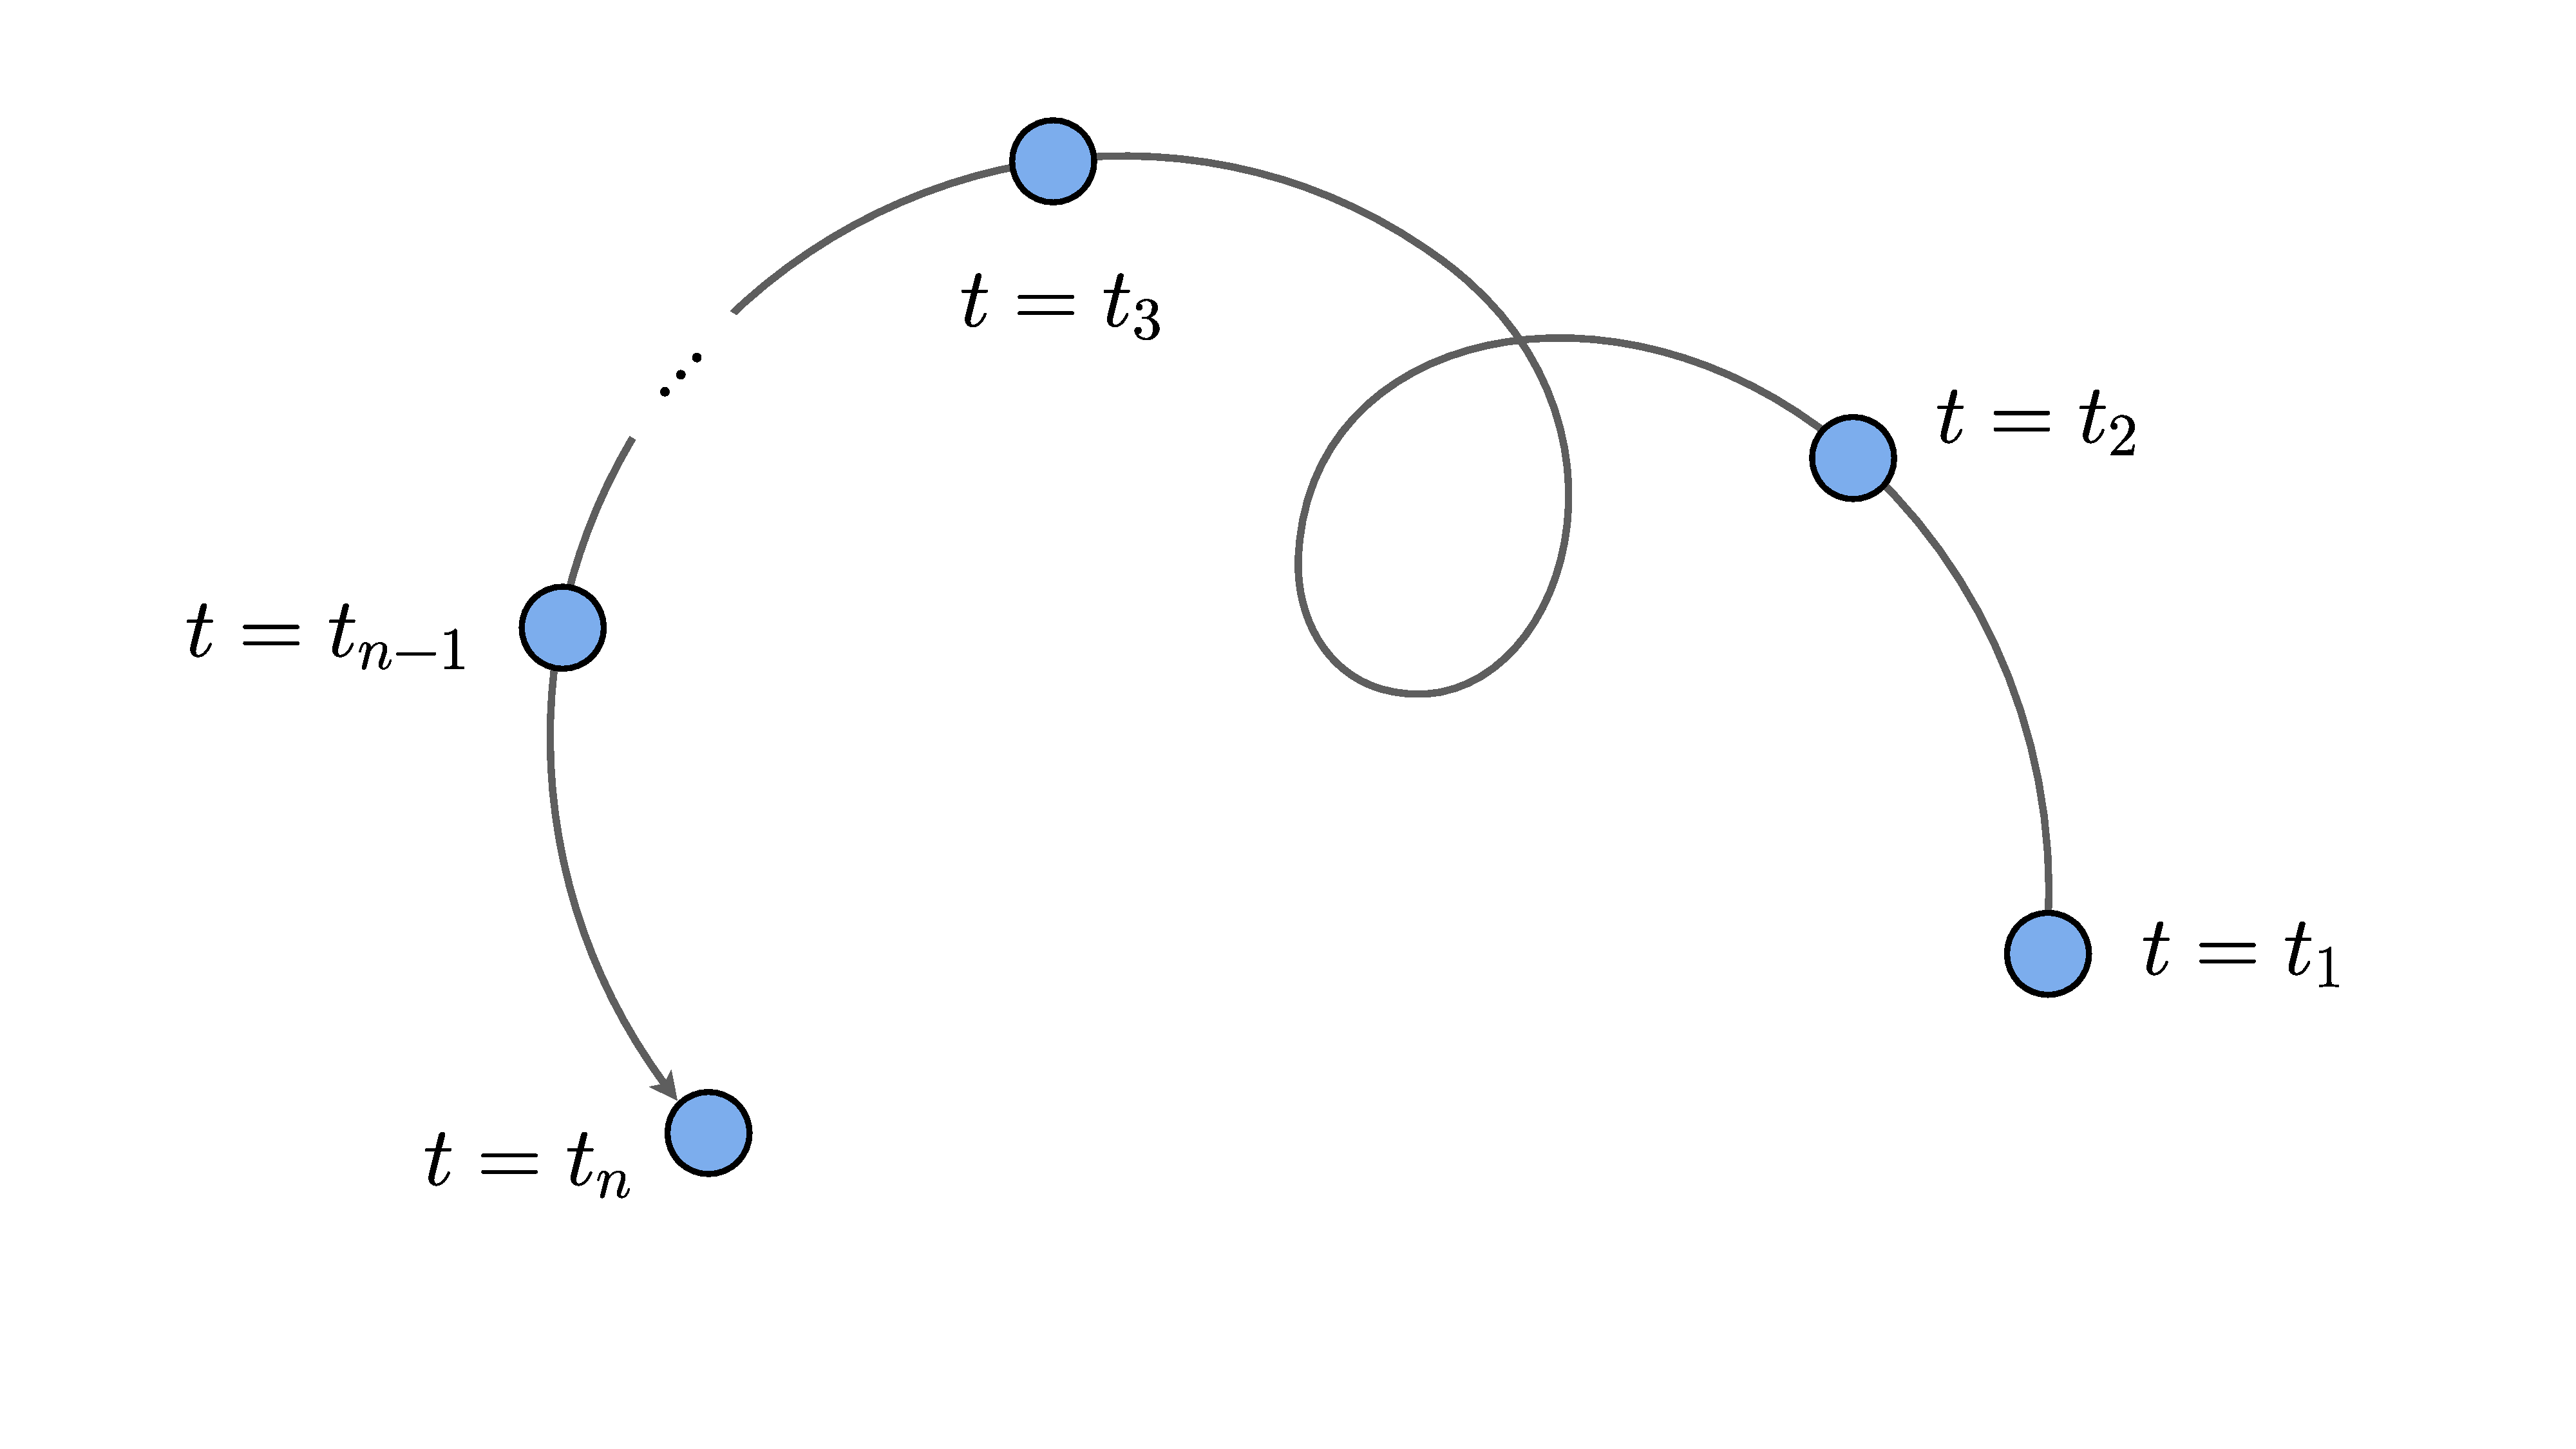
\includegraphics[page=1, width=0.62\linewidth]{imgs.pdf}
    \caption{A moving particle in $\mathbb{R}^2$}
\end{figure}
\end{frame}
%%%%%%%%
\begin{frame}
	However, if we add a coordinate
	\begin{figure}
    \includegraphics[page=2, width=0.62\linewidth]{imgs.pdf}
    %\caption{A moving particle in $\mathbb{R}^2$ with coordinate}
	\end{figure}
	And define the magnitude angular velocity to be
	\begin{equation}
	\omega = \lim_{t_1 \to t_2}\frac{\theta(t_2) - \theta(t_1)}{t_2 - t_1} = \frac{d\theta}{dt}
	\end{equation}
\end{frame}
%%%%%%%%
\begin{frame}
	Notice that, the velocity can be calculated in polar coordinate ($\mathbb{R}^2$)
	by position vector $\vec{r} = r\cos\theta\hat{e}_{x}+ r\sin\theta\hat{e}_y$, that is 
	\begin{equation}
	\begin{aligned}
	\vec{v} &= \frac{d\vec{r}}{dt} 
	= \frac{d}{dt}\left(r\left(\cos\theta\hat{e}_{x}+ \sin\theta\hat{e}_y\right)\right)\\
	&= \frac{dr}{dt} \left(\cos\theta\hat{e}_x + \sin\theta\hat{e}_y\right) 
		+ r\left(-\sin\theta\hat{e}_x + \cos\theta\hat{e}_y\right)\frac{d\theta}{dt}\\
		&= \frac{dr}{dt}\hat{e}_r + r\frac{d\theta}{dt}\hat{e}_\theta
	\end{aligned}
	\end{equation}
	Extending the space to $z$ component, 
	we define the angular velocity for a particle on the $xy$-plane in $\mathbb{R}^3$
	\begin{equation}
	\vec{\omega} = \frac{\hat{e}_r\times \vec{v}}{r} 
	= \frac{r(\hat{e}_{r}\times\hat{e}_\theta)}{r}\frac{d\theta}{dt}
	= \frac{d\theta}{dt} \hat{e}_z,
	\end{equation}
	where $\hat{e}_r$, $\hat{e}_\theta$ and $\hat{e}_z$ are the orthonormal basis of cylinder coordinate.
\end{frame}
%%%%%%%%
\begin{frame}
	Now, consider the particle in $\mathbb{R}^3$ and 
	we still using position vector $\vec{r}$ rather than the $r$-component vector,
	since $\hat{e}_r = \vec{r}/r$, we also can write 
	\begin{equation}
	\vec{\omega} = \frac{\vec{r}\times \vec{v}}{r^2}.
	\end{equation}

	\begin{figure}
    \includegraphics[page=3, width=0.8\linewidth]{imgs.pdf}
	\end{figure}
\end{frame}
%%%%%%%%
\begin{frame}
	Then, how about a group of particles? Average angular velocity?
	\begin{equation}
	\tilde{\Omega} = \frac{1}{n}\sum_{i=1}^{n}\vec{\omega}_i 
	= \sum_{i=1}^{n}\frac{\vec{r}_i\times\vec{v}}{\lVert \vec{r}_i\lVert^2}
	\end{equation}

	\begin{figure}
    \includegraphics[page=4, width=0.65\linewidth]{imgs.pdf}
	\end{figure}
	
	It seems not to be a good estimating method.
\end{frame}
%%%%%%%%
%----
\subsection{Stream line and Path line}
%----
\begin{frame}
\frametitle{Stream line and Path line}
	There are two ways to describe how fluid flow in \textit{Experimental Physics}.
	\begin{figure}
    \includegraphics[page=5, width=0.9\linewidth]{imgs.pdf}
	\end{figure}
\end{frame}
%%%%%%%%
\begin{frame}
	So, a more intuitive way to describe how a group of particles (fluid) rotate,
	is to place a marker is these particles. 
	\begin{figure}
    \includegraphics[page=6, width=0.9\linewidth]{imgs.pdf}
    \caption{The \textit{world line} of marker and vector field}
	\end{figure}
\end{frame}
%%%%%%%%
%----
\subsection{Example}
%----
\begin{frame}
	\frametitle{Example}
	Now, consider a fluid flow given by
	\begin{equation}
	\vec{u}(x,y) = u_x\hat{e}_x + u_y \hat{e}_{y} = -y\,\hat{e}_x + x\,\hat{e}_y
	\end{equation}
	
	\begin{figure}
    \includegraphics[page=7, width=0.9\linewidth]{imgs.pdf}
	\end{figure}
\end{frame}
%%%%%%%%
\begin{frame}
	Using another example fluid flow given by
	\begin{equation}
	\vec{u}(x,y) = \left(y^3 - 9y\right) \hat{e}_x + \left(x^3 - 9x\right)\hat{e}_y
	\end{equation}
	
	\begin{figure}
    \includegraphics[page=8, width=0.8\linewidth]{imgs.pdf}
	\end{figure}

\end{frame}
%%%%%%%%
\begin{frame}
	After we solving the system of non-linear differential equations, we have the path line and moving particles (click \underline{\href{https://youtube.com/shorts/bfFM8ztiRJc?si=1c8Zehqdbq2fMtKz}{here}} to see video). 
	\begin{figure}
	\includegraphics[page=9,width=0.9\textwidth]{imgs.pdf}
    \caption{Left figure is the path line of vector field, reft figure is a snapshot of the simulation video}
	\end{figure}
\end{frame}
%%%%%%%%
\begin{frame}
	\begin{columns}[t]
		\begin{column}{0.5\textwidth}
			Also calculate the curl of vector field
			\begin{equation}
			\begin{aligned}
			\operatorname{curl} \vec{u} 
			&= \partial_{x}(x^3-9x)  - \partial_{y}(y^3-9y)\\
			&=3(x^3-y^2),
			\end{aligned}
			\end{equation}
			and make a contour:
		\end{column}
		\begin{column}{0.5\textwidth}
		\begin{figure}
	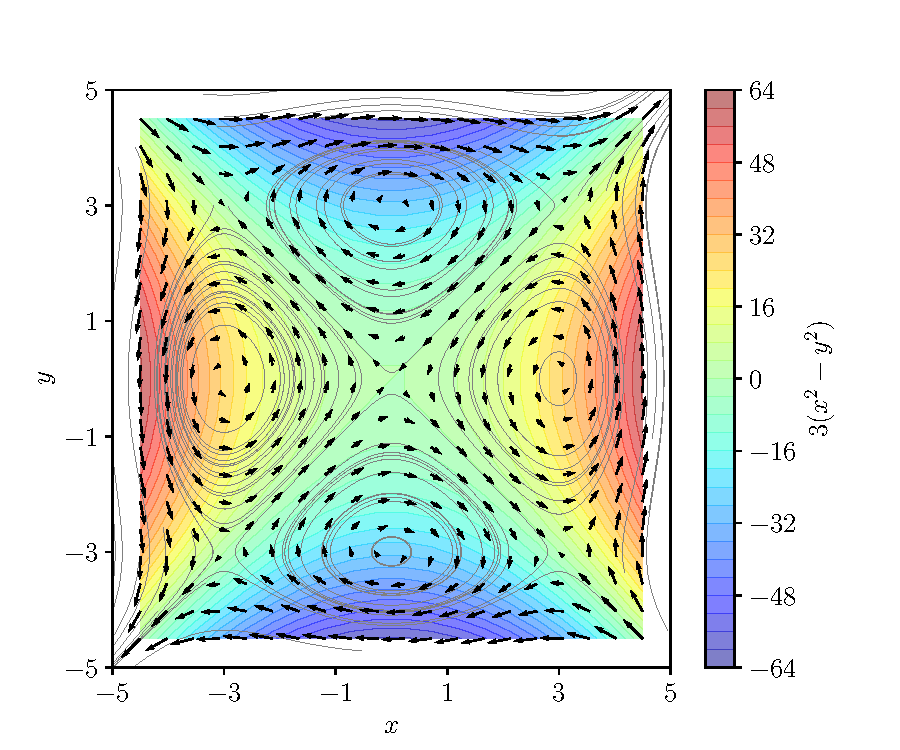
\includegraphics[page=1,width=0.98\textwidth]{flow-countour.pdf}
	\end{figure}
		\end{column}

	\end{columns}
	Here state a conclusion,
	\begin{quote}
	\bigskip
	The curl is to measure the rotation at specific point.
	\end{quote}
\end{frame}
%%%%%%%%
%------------------------------------------------
\section{Circulation and Rotation}
%------------------------------------------------
%----
\subsection{Definition of Circulation}
%----
%%%%%%%%
\begin{frame}
\frametitle{Definition of Circulation}
	Now, consider a simple closed oriented curve $C$ , 
	the \textit{circulation} $\Gamma_C$ of vector field $\vec{u}$ on $C$ is given by
	\begin{equation}
	\Gamma_{C} = \oint_{C}\vec{u}\cdot d\vec{\ell},
	\end{equation}
	where $d\vec{\ell}$ is the infinitesimal displacement vector on $C$.
	More precisely, 
	\begin{block}{Definition of circulation in $\mathbb{R}^2$}
		For a vector field $\vec{u}:S\subseteq \mathbb{R}^2 \to \mathbb{R}^2$,
		given a piecewise smooth oriented curve $C$ parametrized by 
		$\vec{\ell}(t) = x(t)\hat{e}_x + y(t)\hat{e}_y$,
		where $a\leq t\leq b$ and $\vec{\ell}(a)=\vec{\ell}(b)$,
		the circulation $\Gamma$ of $\vec{u}$ on $C$ is given by
		\begin{equation}
		\Gamma_{C} = \oint_{C}\vec{u}\cdot\frac{d\vec{\ell}(t)}{dt}dt 
		= \int_{a}^{b} \vec{u}\left(x(t),y(t)\right)\cdot \frac{d\vec{\ell}(t)}{dt} dt.
		\end{equation}
	\end{block}
\end{frame}
%%%%%%%%
\begin{frame}
	But why are we using circulation ? By Stokes' theorem we have
	\begin{equation}
	\oint_{\partial \Sigma} \vec{u}\cdot d\vec{\ell} 
	= \int_{\Sigma} \left(\operatorname{curl}\vec{u}\right)\cdot d\vec{\Sigma},
	\end{equation}
	where $\ell = \partial \Sigma$ is the boundary of $\Sigma$, 
	and $\Sigma$ is smooth oriented surface.
	If we only consider $\mathbb{R}^2$, we have the circulation
	\begin{equation}
	\Gamma_{\partial \Sigma} = \oint_{\partial \Sigma} \vec{u}\cdot d\vec{\ell} 
	= \iint_{\Sigma} \left(\operatorname{curl}\vec{u}\right)\,dx\,dy.
	\end{equation}
\end{frame}
%----
\subsection{Approximation of circulation}
%----
%%%%%%%%
\begin{frame}
\frametitle{Definition of Circulation}
	Let the area of $\Sigma$ to be $\displaystyle A = \iint_{\Sigma} dxdy$, we have 
	\begin{equation}
	\Gamma_{\partial \Sigma} = A \cdot \frac{\displaystyle\iint_{\Sigma} \left(\operatorname{curl}	\vec{u}\right)\,dx\,dy}{\displaystyle\iint_{\Sigma} dxdy}
	\approx \text{Area}\times\text{mean of $\operatorname{curl}\vec{u}$ in $\Sigma$.}
	\end{equation}
	Here state a conclusion,
	\begin{quote}
	\bigskip
	The circulation is to measure the rotation in a region.
	\end{quote}

\end{frame}
%%%%%%%%
\begin{frame}
	So, now the method to estimate the rotation of the fluid flow with fluid velocity $\vec{u}$ are 
	\begin{enumerate}
	\item Curl $\nabla \times \vec{u}(\vec{r}) = \operatorname{curl}\vec{u}(\vec{r})$ is to measure the rotation at point $\vec{r}$.
	\item Circulation $\displaystyle \Gamma_{C} = \oint_{C}\vec{u}\cdot d\vec{\ell}$ is to measure the rotation in a region $C$.
	\end{enumerate}
	So, now let us consider some special case for $\nabla\times\vec{\vec{u}}=0$. 
\end{frame}
%%%%%%%%
%------------------------------------------------
\section{Curl and Circulation}
%------------------------------------------------
%----
\subsection{Vector calculus}
%----
%%%%%%%%
\begin{frame}
\frametitle{Vector calculus}
	First, let us specify our coordinates, that is
	\begin{figure}
	\includegraphics[page=10,width=1.0\textwidth]{imgs.pdf}
	\end{figure}
\end{frame}
%%%%%%%%
\begin{frame}
	The curl in three different coordinate are
	\begin{enumerate}
	\item For a vector field $\vec{A} = A_x \hat{e}_x + A_y \hat{e}_y + A_z \hat{e}_z$
		\begin{equation}
		\nabla \times \vec{A} = 
		\begin{vmatrix}
		\hat{e}_x & \hat{e}_y & \hat{e}_z\\
		\partial_x & \partial_y & \partial_z\\
		A_x & A_y & A_z
		\end{vmatrix}
		\end{equation}
	\item For a vector field $\vec{A} = A_r \hat{e}_r + A_\theta \hat{e}_\theta + A_z \hat{e}_z$
		\begin{equation}
		\nabla \times \vec{A} = 
		\begin{vmatrix}
		\hat{e}_r & r\hat{e}_\theta & \hat{e}_z\\
		\partial_r & \partial_\theta & \partial_z\\
		A_r & r A_\theta & A_z
		\end{vmatrix}
		\end{equation}
	\item For a vector field $\vec{A} = A_r \hat{e}_r + A_\theta \hat{e}_\theta + A_\varphi \hat{e}_\varphi$
		\begin{equation}
		\nabla \times \vec{A} = 
		\frac{1}{r^2\sin\theta}\begin{vmatrix}
		\hat{e}_r & r\hat{e}_\theta & r\sin\theta\,\hat{e}_\varphi\\
		\partial_r & \partial_\theta & \partial_z\\
		A_r & r A_\theta & r\sin\theta\,A_z
		\end{vmatrix}
		\end{equation}
	\end{enumerate}
	Or, expanding ...
\end{frame}
%%%%%%%%
\begin{frame}
	\begin{enumerate}
	\item For a vector field $\vec{A} = A_x \hat{e}_x + A_y \hat{e}_y + A_z \hat{e}_z$
		\begin{equation}\small
		\nabla\times\vec{A} = 
		\left(\frac{\partial A_z}{\partial y} - \frac{\partial A_y}{\partial z}\right)\hat{e}_x
		- \left(\frac{\partial A_z}{\partial x}  - \frac{\partial A_x}{\partial z}\right)\hat{e}_y
		+ \left(\frac{\partial A_y}{\partial x}  - \frac{\partial A_x}{\partial y}\right)\hat{e}_z
		\end{equation}
	
	\item For a vector field $\vec{A} = A_r \hat{e}_r + A_\theta \hat{e}_\theta + A_z \hat{e}_z$
		\begin{equation}\small
		\nabla \times \vec{A} =
		\left(\frac {1}{r}\frac{\partial A_z}{\partial \theta}
			-\frac{\partial A_\theta}{\partial z}\right) \hat{e}_r
		+\left(\frac {\partial A_r}{\partial z}
			-\frac {\partial A_z}{\partial r}\right) \hat{e}_\theta
		+\frac{1}{r}\left(\frac {\partial}{\partial r}\left(r A_\theta\right)
			-\frac{\partial A_r}{\partial \theta}\right)\hat{e}_z
		\end{equation}

	\item For a vector field $\vec{A} = A_r \hat{e}_r + A_\theta \hat{e}_\theta + A_\varphi \hat{e}_\varphi$
		\begin{equation}\small
		\begin{aligned}
		\nabla\times\vec{A} &=
		\frac{1}{r\sin\theta}\left(\frac{\partial}{\partial \theta}\left(A_z \sin\theta\right)
			-\frac{\partial A_\theta}{\partial \varphi}\right)\hat{e}_r\\
		&\quad + \frac{1}{r}\left(\frac{1}{\sin\theta}\frac{\partial A_r}{\partial \varphi} 
			- \frac{\partial}{\partial r}\left(rA_{\varphi}\right)\right)\hat{e}_\theta
		+ \frac{1}{r}\left(\frac{\partial}{\partial r}\left(r A_\theta\right)
			- \frac{\partial A_{r}}{\partial \theta}\right)\hat{e}_\varphi
		\end{aligned}
		\end{equation}
	\end{enumerate}
\end{frame}
%----
\subsection{Example for Cartesian}
%----
%%%%%%%%
\begin{frame}
\frametitle{Example for Cartesian}
	\begin{columns}[t]
		\begin{column}{0.5\textwidth}
			Here, for simplicity, we only consider the flow on the $xy$-plane 
			and using the Cartesian coordinate to describe. We consider a flow velocity 
			\begin{equation}
			\vec{u}(x,y) = 1\cdot \hat{e}_x.
			\end{equation}
			Obviously, the curl is zero, $\nabla\times\vec{u} = 1$, 
			since it is a uniform flow.
		\end{column}
		\begin{column}{0.5\textwidth}
			\begin{figure}
			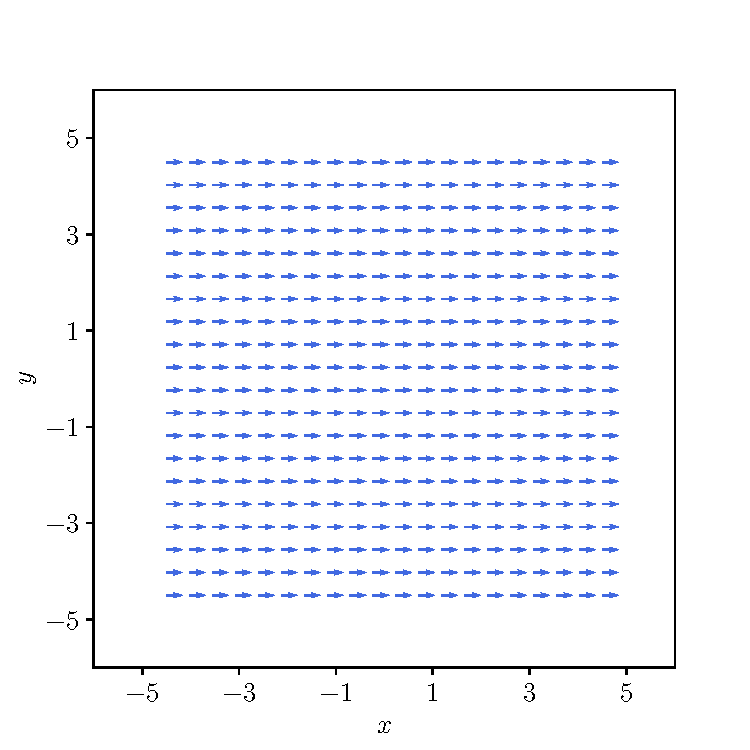
\includegraphics[page=1, width=1.0\textwidth]{flow-(1,0).pdf}
			\end{figure}
		\end{column}
	\end{columns}
\end{frame}
%%%%%%%%
\begin{frame}
	\begin{columns}[t]
		\begin{column}{0.5\textwidth}
			Another example is to consider the flow velocity 
			\begin{equation}
			\vec{u}(x,y) = -y\cdot \hat{e}_x,
			\end{equation}
			so that the velocity grows when $y$ becomes larger. Now, the curl is 
			\begin{equation}
			\nabla\times\vec{u} = 1 \cdot \hat{e}_z,
			\end{equation}
			Although, the curl is not zero, 
			we still can not see any rotation in the arrow graph of  vector field.
		\end{column}
		\begin{column}{0.5\textwidth}
			\begin{figure}
			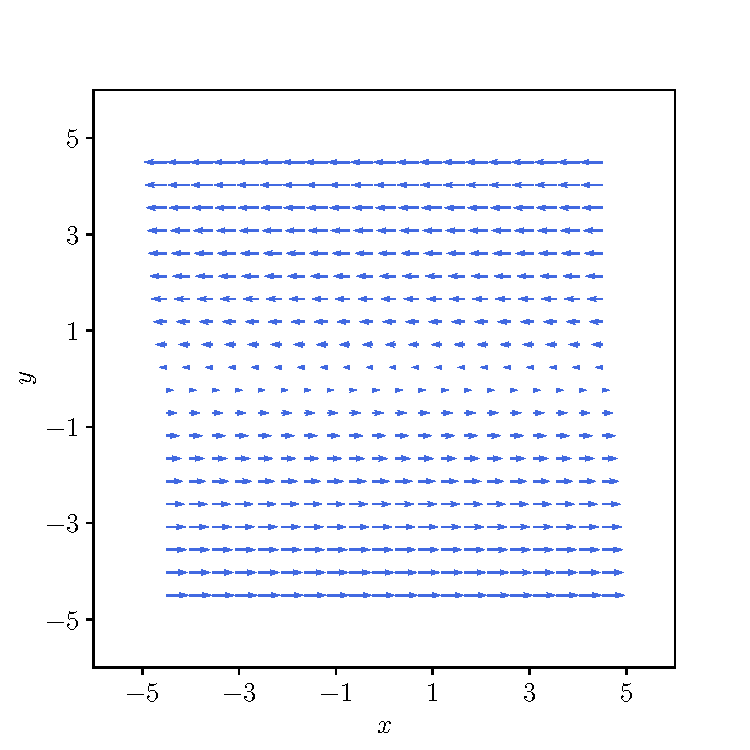
\includegraphics[page=1, width=1.0\textwidth]{flow-(-y,0).pdf}
			\end{figure}
		\end{column}
	\end{columns}
\end{frame}
%%%%%%%%
\begin{frame}
Even the stream and path line, we still cannot see any rotation.
	\begin{columns}[t]
		\begin{column}{0.5\textwidth}
			\begin{figure}
			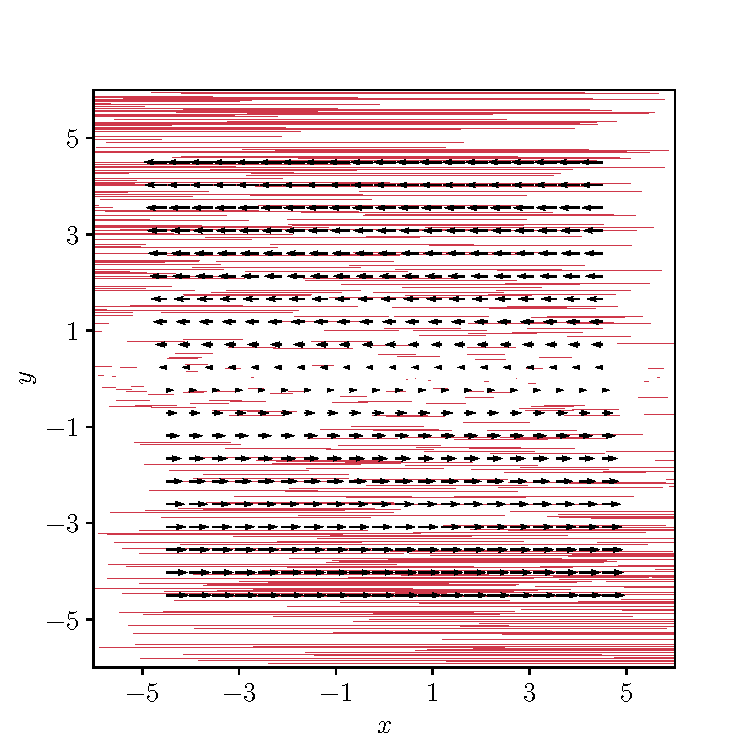
\includegraphics[page=1, width=0.9\textwidth]{flow-(-y,0)-path.pdf}
			\caption{Given random initial position condition to solve \textit{path line}.}
			\end{figure}
		\end{column}
		\begin{column}{0.5\textwidth}
			\begin{figure}
			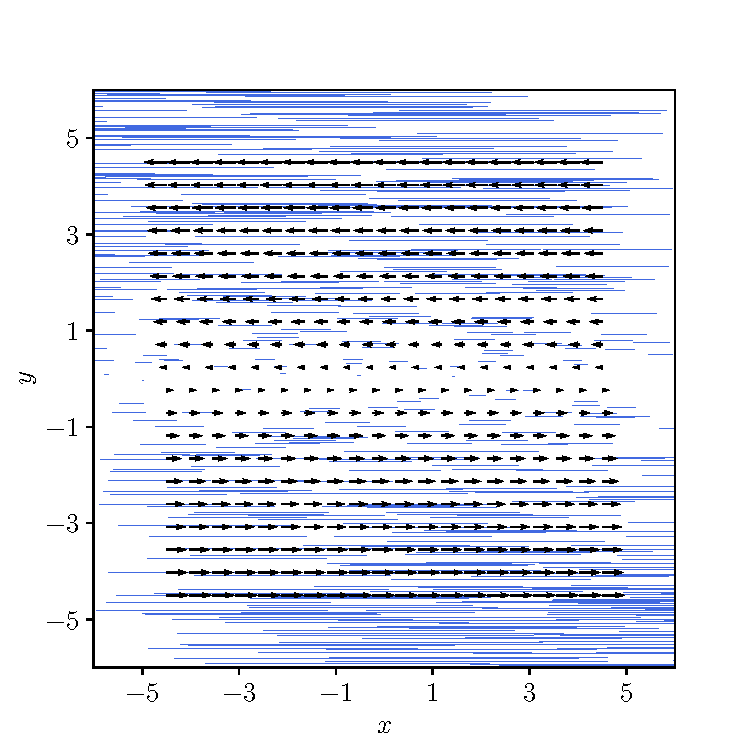
\includegraphics[page=1, width=0.9\textwidth]{flow-(-y,0)-stream.pdf}
			\caption{Given random initial position condition to solve \textit{stream line}.}
			\end{figure}
		\end{column}
	\end{columns}
\end{frame}
%%%%%%%%
\begin{frame}
	But if we look at some specific particle in space:
	\begin{columns}[t]
		\begin{column}{0.5\textwidth}
			\begin{figure}
			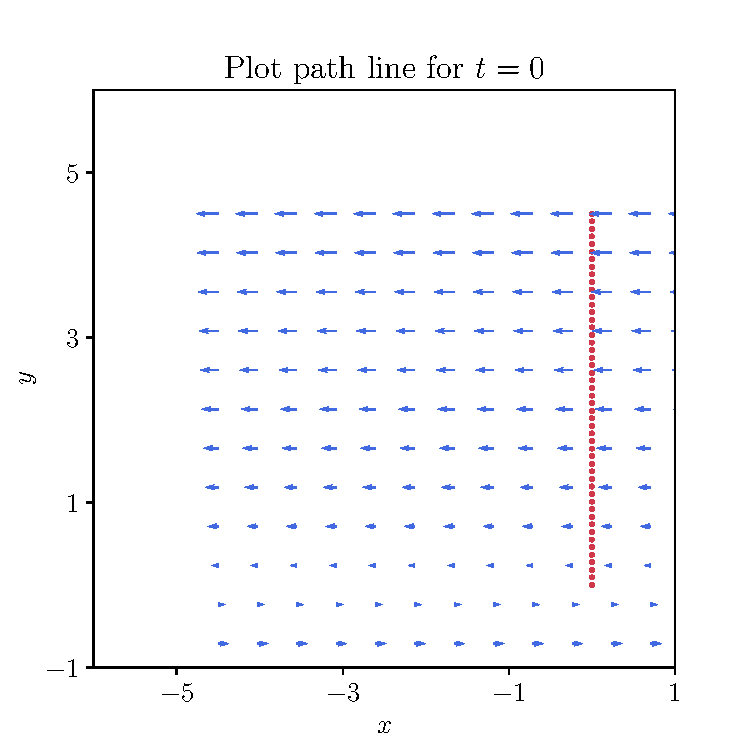
\includegraphics[page=1, width=0.9\textwidth]{flow-(-y,0)-path-initial.pdf}
			\end{figure}
		\end{column}
		\begin{column}{0.5\textwidth}
			\begin{figure}
			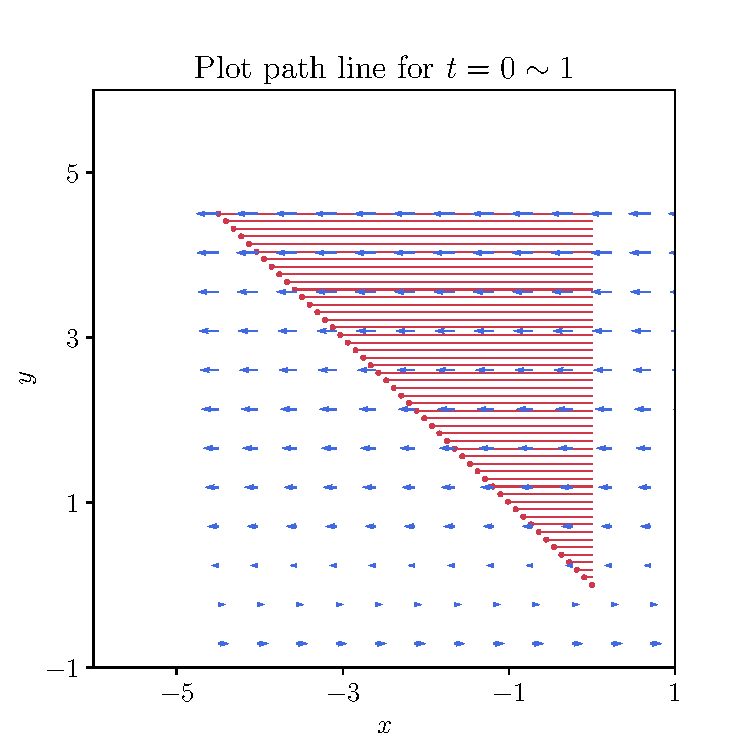
\includegraphics[page=1, width=0.9\textwidth]{flow-(-y,0)-path-final.pdf}
			\end{figure}
		\end{column}
	\end{columns}
\end{frame}
%%%%%%%%
\begin{frame}
	And link the particles in each time, and color them in different colors: 
	\begin{columns}[t]
		\begin{column}{0.49\textwidth}
			\begin{figure}
			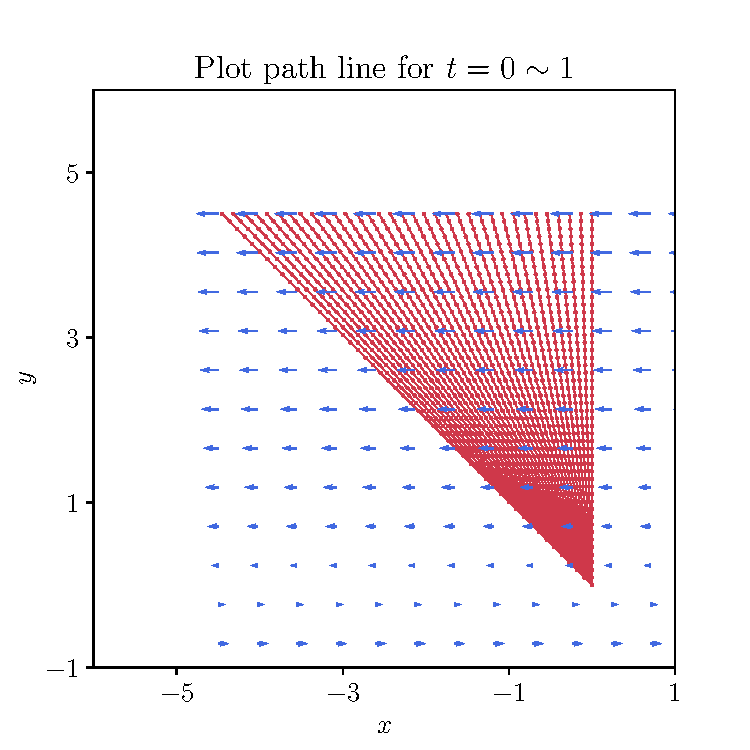
\includegraphics[page=1, width=0.9\textwidth]{flow-(-y,0)-path-links.pdf}
			\end{figure}
		\end{column}
		\begin{column}{0.51\textwidth}
			\begin{figure}
			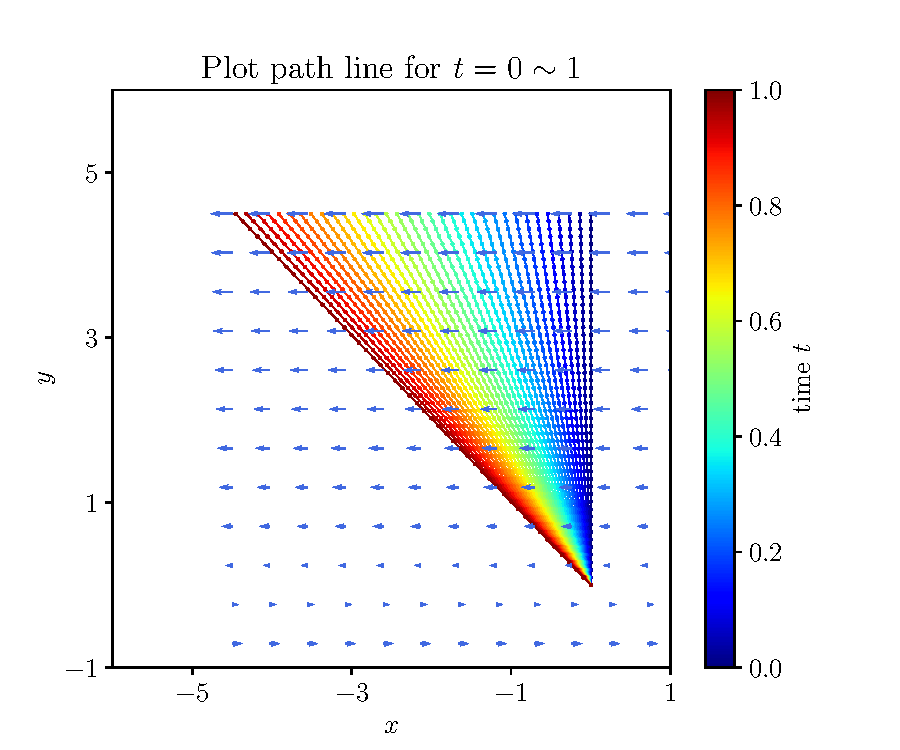
\includegraphics[page=1, width=1.0\textwidth]{flow-(-y,0)-path-color.pdf}
			\end{figure}
		\end{column}
	\end{columns}
\end{frame}
%%%%%%%%
\begin{frame}
	Here, for simplicity, we only consider the flow on the $xy$-plane and 
	using the cylindrical coordinate to describe. So, the fluid velocity now becomes
	\begin{equation}
	\vec{u}(r,\theta) = u_r(r,\theta) \hat{e}_r + u_\theta (r,\theta) \hat{e}_\theta,
	\end{equation}
	and then the curl
	\begin{equation}\small
		\nabla \times \vec{u} =
		\left(\frac {1}{r}\frac{\partial u_z}{\partial \theta}
			-\frac{\partial u_\theta}{\partial z}\right) \hat{e}_r
		+\left(\frac {\partial u_r}{\partial z}
			-\frac {\partial u_z}{\partial r}\right) \hat{e}_\theta
		+\frac{1}{r}\left(\frac {\partial}{\partial r}\left(r u_\theta\right)
			-\frac{\partial u_r}{\partial \theta}\right)\hat{e}_z
	\end{equation}
	becomes
	\begin{equation}
	\nabla \times \vec{u} = \frac{1}{r}\left(\frac {\partial}{\partial r}\left(r u_\theta\right)
		-\frac{\partial u_r}{\partial \theta}\right)\hat{e}_z,
	\end{equation}
	also notice that the differential displacement in this case is 
	\begin{equation}
	d\vec{\ell} = dr\,\hat{e}_{r} + rd\theta\,\hat{e}_{\theta}.
	\end{equation}

\end{frame}
%%%%%%%%
%----
\subsection{Example for Cylindrical}
%----
\begin{frame}
\frametitle{Example for Cylindrical}
	Now, let $\vec{u}(r,\theta) = u_\theta(r,\theta)\hat{e}_\theta$, 
	and solve for $0=\nabla\times\vec{u}$, we have
	\begin{align}
	& 0 = \frac{1}{r}\left(\frac {\partial}{\partial r}\left(r u_\theta(r,\theta)\right)
		-\frac{\partial 0}{\partial \theta}\right)\hat{e}_z\\
	\Rightarrow\quad 
	& 0 = u_\theta(r,\theta) + r\frac{\partial u_{\theta}(r,\theta)}{\partial r},
	\quad\text{for $r\neq 0$}\\
	\Rightarrow\quad 
	& \frac{\partial u_{\theta}(r,\theta)}{\partial r} = -\frac{u_{\theta}(r,\theta)}{r}.
	\end{align}
	By experience, the general solution is $u_{\theta}(r,\theta) = r^{-1}f(\theta)$, 
	where $f$ is a function of $\theta$. We can check by plug into the equation
	\begin{equation*}
	\frac{\partial u_{\theta}(r,\theta)}{\partial r} 
	= -r^{-2}f(\theta) 
	= -\frac{r^{-1}f(\theta)}{r} 
	= -\frac{u_{\theta}(r,\theta)}{r}.
	\end{equation*}
\end{frame}
%%%%%%%%
\begin{frame}
	Then we can calculate the circulation for 
	$\vec{u}(r,\theta) = u_\theta(r,\theta)\hat{e}_\theta$ such that $\nabla \times \vec{u}= 0$, 
	the general solution is $u_\theta(r,\theta) = r^{-1}f(\theta)$, 
	then the circulation in cylindrical coordinate (polar coordinate) is 
	\begin{align}
	\Gamma_{C} = \oint_{C}\vec{u}\cdot d\vec{\ell} = \oint_{C} u_{\theta}(r,\theta)\,rd\theta
	= \oint_{C} f(\theta) d\theta.
	\end{align}
	Now, we can observing that, although the curl is zero, if $f(\theta)>0$ on $C$, then $\Gamma_{C}>0$, on the other hand, if $f(\theta)<0$ on $C$, then $\Gamma_{C}<0$.
\end{frame}

%%%%%%%%
\begin{frame}
	Now, consider a more general case, 
	let $\vec{u}(r,\theta) = u_r(r,\theta)\hat{e}_r + u_\theta(r,\theta)\hat{e}_\theta$, 
	and solve for $\nabla\times \vec{u} = 0$, we have
	\begin{equation}
	0 = \frac {\partial}{\partial r}\left(r u_\theta(r,\theta)\right)
		-\frac{\partial u_r(r,\theta)}{\partial \theta},
	\end{equation}
	Also, by experience, let $u_{r}(r,\theta) = r^{-1}f(r,\theta)$, we have
	\begin{equation}
	\frac{\partial f(r,\theta)}{\partial r} = \frac{\partial u_r(r,\theta)}{\partial \theta},
	\end{equation}
	which is the first equation in \textit{Cauchy–Riemann equations}.
\end{frame}

%%%%%%%%
\begin{frame}
	In order to solve $\partial f(r,\theta)/\partial r = \partial u_r(r,\theta)/\partial \theta$, 
	we can suppose there exists a potential function $\phi(r,\theta)$ such that 
	\begin{equation}
	f(r,\theta) = \frac{\partial \phi(r,\theta)}{\partial \theta}
	\quad \text{and}\quad
	u_{r}(r,\theta) = \frac{\partial \phi(r,\theta)}{\partial r}.
	\end{equation}
	With this assumption, the equation is automatically satisfied:
	\begin{equation*}
	\frac{\partial f(r,\theta)}{\partial r} 
	= \frac{\partial^2 \phi(r,\theta)}{\partial r \partial \theta}
	= \frac{\partial^2 \phi(r,\theta)}{\partial \theta \partial r}
	= \frac{\partial u_r(r,\theta)}{\partial \theta}.
	\end{equation*}
	Now, the solution is 
	\begin{equation}
	\vec{u} = \frac{\partial \phi(r,\theta)}{\partial r} \hat{e}_{r} 
			  + \frac{1}{r}\frac{\partial \phi(r,\theta)}{\partial \theta} \hat{e}_{r} = \nabla\phi
	\end{equation}
	where $\phi$ is any function of $r$ and $\theta$.
\end{frame}

%%%%%%%%
\begin{frame}
	Then we can calculate the circulation for 
	$\vec{u} = u_r(r,\theta)\hat{e}_r + u_\theta(r,\theta)\hat{e}_\theta$ 
	such that $\nabla \times \vec{u}= 0$.
	The general solution is $u_\theta(r,\theta) = \partial_{r}\phi\,\hat{e}_{r} + r^{-1}\partial_\theta \phi\,\hat{e}_{r} $, where $\phi$ is any function of $r$ and $\theta$. The circulation in cylindrical coordinate (polar coordinate) is 
	\begin{align}
	\Gamma_{C} 
	&= \oint_{C}\vec{u}\cdot d\vec{\ell} = \oint_{C} \bigg(u_{r}(r,\theta)dr + u_{\theta}(r,\theta)\,rd\theta\bigg)\\
	&= \oint_{C} \frac{\partial \phi(r,\theta)}{\partial r} dr + \frac{1}{r}\frac{\partial \phi(r,\theta)}{\partial \theta} rd\theta\\
	&= \oint_{C} \frac{\partial \phi(r,\theta)}{\partial r} dr + \frac{\partial \phi(r,\theta)}{\partial \theta} d\theta\\
	&= \oint_{C} \nabla\phi\cdot d\vec{\ell} =\oint_{C}d\phi,
	\end{align}
	where $d\phi$ is the total differential.
\end{frame}
%%%%%%%%
\begin{frame}
	Usually, $\phi$ is a continuous function; however, not always. 
	If a piecewise smooth oriented path $C$ can be parameterized by
	\begin{equation}
	\vec{\ell}(t) = x(r(t),\theta(t))\hat{e}_{x} + y(r(t),\theta(t))\hat{e}_{y},
	\end{equation}
	where $t\in[a,b]$ and $\vec{\ell}(a) = \vec{\ell}(b)$, then the circulation becomes
	\begin{equation}
	\Gamma_{C} = \phi(\vec{r}(b)) - \phi(\vec{r}(a)).
	\end{equation}
	However, if $\phi(r,\theta) = \theta$, 
	the vector field is $\vec{u}=\nabla\phi = 1/r \hat{e}_{\theta}$. 
	If the path $C$ surrounds the origin, which is the pole $r=0$, 
	the circulation becomes $\Gamma_C = 2\pi - 0 = 2\pi > 0$, 
	which means the circulation still can be measurement of rotation.

\end{frame}
%%%%%%%%
%------------------------------------------------
\section{Conclusion}
%------------------------------------------------
\begin{frame}
	Here, I list some potential function $\phi$ in cylindrical coordinate, so that $\nabla\times\vec{u}=0$:
	\begin{table}[t]
	\begin{tabular}{c|c|c|c}
	$\phi(r,\theta)$	&	$\vec{u}=\nabla \phi$	& 	$\nabla \times \vec{u}$ & $\Gamma_{C}$ \\\hline\hline
	$\theta$	& 	$\displaystyle \left(1/r\right) \hat{e}_{\theta}$&$0$&$\neq 0$\\\hline
	$c_0+c_1\cdot\theta$	& 	$ \left(c_1/r\right) \hat{e}_{\theta}$&$0$&$\neq 0$\\\hline
	$\sum_{s=0}^{n}c_{s}\cdot\theta^{s}$	& $\left(\sum_{s=1}^{n}sc_{s}\cdot\theta^{s-1}/r\right) \hat{e}_{\theta}$&$0$&$\neq 0$\\\hline
	$f(\theta)$	& 	$\left(f'(\theta)/r\right) \hat{e}_{\theta}$	&	$0$ & ?\\\hline
	$g(r)\cdot f(\theta)$	& 	$\left(g'(r) f(\theta)\right) \hat{e}_{r} + \left(g(r) f'(\theta)/r\right) \hat{e}_{\theta}$	&	$0$  & ?\\\hline
	$\vdots$	& 	$\vdots$	&	$0$  & $\vdots$\\
	\end{tabular}
	\end{table}
	where $c_0,c_1,\ldots,c_n$ are constants, and $f$ is any function of $\theta$, $g$ is any function of $r$. 
\end{frame}
%%%%%%%%
\begin{frame}
\frametitle{Conclusion}
In conclude, 
\begin{enumerate}
\item The \textbf{\textit{curl}} is to measure the rotation at specific point. 
\item The \textbf{\textit{circulation}} is to measure the rotation in a region.
\item If the potential function is discontinuous on the closed path, even if curl is zero, the circulation can still be nonzero.
\end{enumerate}
\end{frame}
%%%%%%%%
\begin{frame}
	\begin{center}
		\bigskip\bigskip\bigskip
		{\Huge Thanks!}
		
		\bigskip\bigskip
		
		{\LARGE Questions? Comments?}
	\end{center}
\end{frame}
%------------------------------------------------


%----------------------------------------------------------------------------------------

\end{document} 